\section{Qu'est ce que le reconnaissance de formes ?}

La \textbf{Reconnaissance de forme}, ou \textit{Shape Matching} en anglais, est la discipline scientifique dont l'objet d'étude est l'ensemble des méthodes et techniques permettant d'identifier un \textbf{\textit{motif}} et d'en déterminer par la suite la catégorie. C'est un domaine très lié aux méthodes dites de \textbf{Vision par Ordinateur}, ou \textit{Computer Vision} en anglais.

Ses applications sont très larges et vont de la voiture autonome qui doit pouvoir identifier un vaste ensemble de formes variées (panneaux, signalisation au sol, véhicules, personnes, animaux, obstacles ...), au contrôle qualité partiellement ou totalement automatisé.

De manière plus large, on retrouve également ce type d'algorithme en sécurité informatique ou sécurité civile pour détecter un \textit{motif de comportement anormal} : détection d'intrusion réseau, lutte anti-terrorisme \ldots

 \begin{figure}[H]
    \centering
    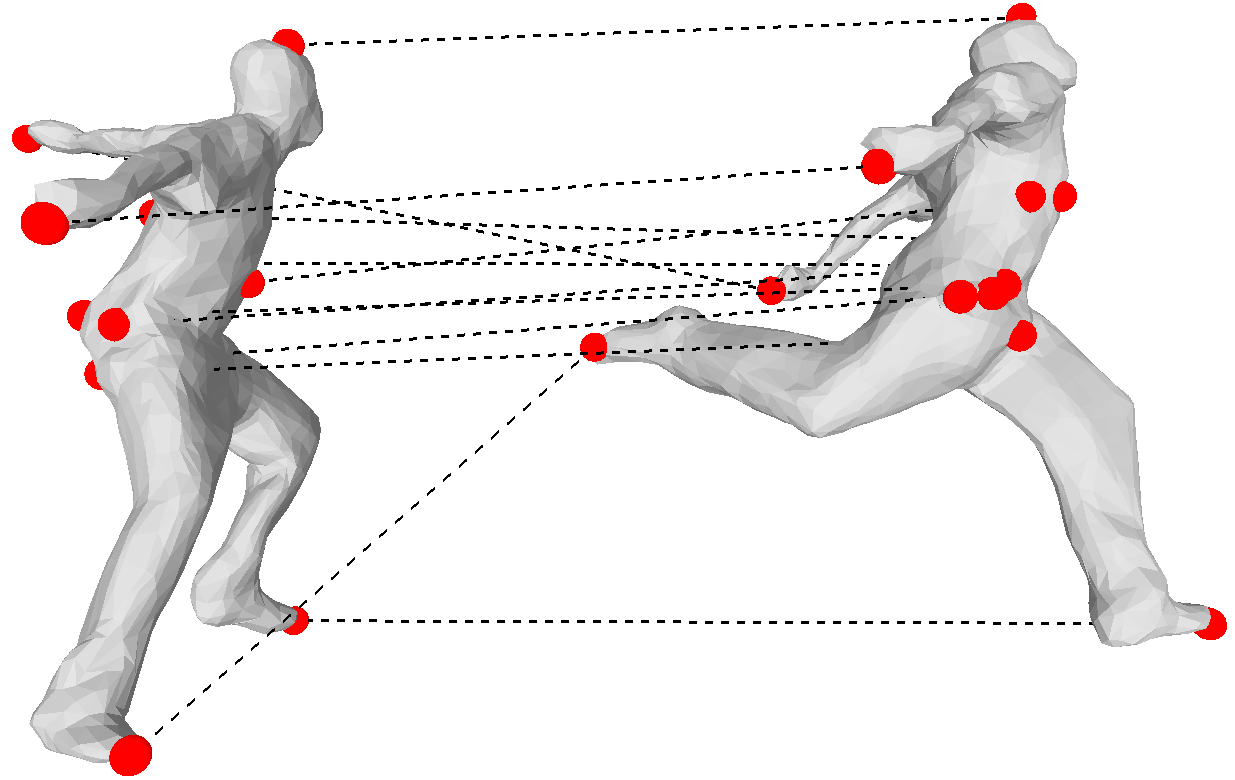
\includegraphics[height=6cm]{shapeMatching.png}
	\caption{Sortie typique d'un algorithme de reconnaissance de formes 2D/3D~\cite{shapeMatchingImg}}\label{image.shapeMatching} 
\end{figure}

 \begin{figure}[H]
    \centering
    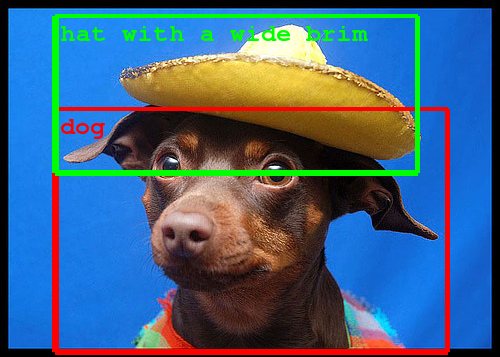
\includegraphics[height=6cm]{computerVision.png}
	\caption{Sortie typique d'un algorithme de vision par ordinateur~-~Source: \href{http://googleresearch.blogspot.fr/2014/09/building-deeper-understanding-of-images.html}{Google Research}}\label{image.computerVision} 
\end{figure}

\section{IaaS vs PaaS vs SaaS vs STaaS}

Quand on parle d'un ``Service Cloud", il y a trois catégories possibles :

\begin{itemize}
	\item \textbf{Infrastructure as a Service (IaaS):}\\ 
	
	Dans ce type d'architecture, \emph{\textbf{le fournisseur}} du service s'engage à livrer et maintenir le serveur, son OS (virtuel ou non), le stockage et le réseau nécessaire.\\
			
	Il reste à la charge \emph{\textbf{du client}} la gestion de la \textit{plateforme} et des diverses applications qui fonctionnent sur cette dernière, les bases de données et les différents logiciels installés.\\
	
	Ce type de service est grandement utile aux entreprises désireuses de revendre des services Cloud type Saas ou Paas de louer des infrastructures hautement flexibles. Pour ne citer que quelques exemples voici quelques fournisseurs de IaaS :\emph{ Cloud Power, DotRiver, Amazon EC2, Windows Azure, Rackspace,~...}\\
			\vspace{8mm}
			
		
	\item \textbf{Platform as a Service (PaaS):}\\
	
	Dans ce type d'architecture, \emph{\textbf{le fournisseur}} du service s'engage à livrer et maintenir tout ce qui compose l'IaaS. A celà s'ajoute en plus la partie plateforme cloud, les bases de données, et les logiciels nécessaires au fonctionnement de la plateforme ou de l'administration du serveur.\\
			
	Il ne reste à la charge \emph{\textbf{du client}} que la gestion des \textit{applications} (et leur dévelopement au besoin) sur la plateforme cloud fournie.\\

Ce type de service est généralement destiné aux utilisateurs finaux, et sont utilisés par de plus en plus de personnes ayant des besoins spécifiques et ne voulant déployer de gros moyens à chaque nouveau projet (petit ou grand) : On retrouvera dans les plateformes : \emph{Force.com pour SalesForce, Google AppEngine, Cordys Process Factory} (sur lequel j'ai travaillé), Microsoft Azure \emph{...}\\
			\vspace{8mm}
	
	
	\item \textbf{Software as a Service (SaaS):}\\
	
	Le Software as a service (SaaS) est l’ultime modèle de Cloud, où \textbf{le fournisseur} Cloud 
maintient absolument tout et developpe les applications.\\
	
	Le \textbf{client} lui est simple ``\emph{utilisateur}" des applications.\\
	
	Ainsi nous retrouvons les applications clouds suivantes en tant que SaaS: \emph{Google Document, Google SpreadSheet, ... }\\
			\vspace{8mm}

\item \textbf{Storage as a Service (STaaS):}\\

 Très similaire au SaaS, seulement cette fois-ci le client ne veut pas une application mais un espace de stockage.\\
 
 \emph{Services Connus : Google Drive, Dropbox, iCloud, Microsoft Skydrive,} ...

\end{itemize}
			\vspace{2cm}
 
\begin{figure}[H]
    \centering
    \includegraphics[height=14cm]{aas.png}
	\caption{IaaS vs PaaS vs SaaS}\label{image.aas} 

\end{figure}